%--------------------------------------------------------------------------------------
% Este arquivo contém a sua metodologia
%--------------------------------------------------------------------------------------
\chapter{Materiais e Métodos} \label{ch:MM} %Uma label é como você referencia uma seção no texto com a tag \ref{}
Neste capítulo apresenta-se as etapas de modelagem e simulação de um braço robótico com 4 graus de
liberdade em estrutura de cadeia fechada no CoppeliaSim. Além disso, apresentam-se os parâmetros de DH para a modelagem cinemática no RTB. Então estabelecendo comunicação entre essas duas ferramentas, verificar a fidelidade dos modelos.

\section{Modelagem}

Para começar a modelagem e simulação de um braço robótico com geometria em paralelo, primeiro foi necessário obter os arquivos de malha (mesh) do protótipo.

O protótipo escolhido foi o EEzyBot Arm MK2, desenvolvido pelo italiano Carlo Franciscone (@daGHIZmo no Thingiverse). Se trata de um manipulador robótico do tipo cotovelo com geometria em paralelogramo. Possui três cadeias cinemáticas fechadas em sua estrutura. No site do repositório desse projeto encontram-se os arquivos STL para fácil impressão em 3D,e o autor também compartilhou o link para os arquivos fontes CAD no OneShape que é um \textit{software as a service}, onde pelo navegador de internet se tem uma completa e poderosa ferramenta CAD. No OneShape foi possível exportar esse modelo em um arquivo 3D do tipo .obj. Em posse desse arquivo, basta importá-lo para o CoppeliaSim (Fig. \ref{img:import.png}).

\imagem{0.4}{import.png}{Janela de import de mesh no CoppeliaSim.}{Autoria própria}

Quando se importa um arquivo de malha para o Coppelia, é provável que a malha desse modelo seja de grande definição de detalhes e formas, e isso prejudica a performance da simulação. O próprio software possui ferramentas para diminuir a quantidade de triângulos da malha (função \textit{decimate} Fig. \ref{img:decimate.png}). Triângulo é a forma geométrica básica da qual toda a malha é feita, quanto mais triângulos, mais detalhes de forma. Reduzindo a quantidade de triângulos em 15\% foi suficiente para ter um número aceitável de formas básicas sem prejudicar a identificação visual das partes do modelo e nem o processamento da simulação.

\imagem{0.4}{decimate.png}{Janela de Decimate mesh no CoppeliaSim.}{Autoria própria}

Agora com a função divide (Fig. \ref{img:divide.png}), o programa automaticamente divide aquele que era uma forma única compreendendo todo o protótipo em partes individuais deste protótipo, com seus elos e engrenagens. Porém sem as juntas que o compõem nem a hierarquia das juntas e seus elos. Após o uso da função divide, muitas partes desnecessárias foram removidas, como: tampa da base, rolamentos, engrenagens, motores e a ferramenta de uso que é uma garra, sobrando apenas os elos e a base em si. Também foram dados nomes aos elos, de forma a facilitar a identificação das partes do modelo e ainda, selecionando todos os elos, duas edições precisaram ser feitas: o frame de referencia da forma foi realocado para o centro da mesh e sua \textit{bounding box} (caixa delimitadora) foi alinhada com o mesh. Prosseguindo assim cada forma possui uma posição de acordo com o World Frame (ou em relação à forma pai); e o tamanho da forma pode ser melhor calculado pela \textit{bounding box}.

\imagem{0.4}{divide.png}{Modelo após aplicar função \textit{divide} no CoppeliaSim.}{Autoria própria}

Então é preciso adicionar juntas à cena. Todas as juntas são do tipo de revolução. Tamanhos e diâmetros foram arbitrados de forma coerente com o modelo. A posição das juntas se faz de forma visual, posicionando no espaço que seria do motor ou parafuso de eixo do modelo real. Então quatro juntas farão o papel de motores do robô, enquanto as outras juntas serão juntas passivas auxiliares.

É preciso definir a hierarquia que define como os elos e juntas estão relacionados. Por se tratar de um modelo com geometria em paralelogramo, com cadeias cinemáticas fechadas, certos elos possuem duas ou mais juntas. O próprio software possui como um modelo embutido o manipulador uArm que possui geometria muito semelhante. Desta forma, espelhar sua hierarquia poderia resolver a questão. Porém a simulação não ocorria de forma adequada. Após estudos e pesquisas, o canal no YouTube do professor da Universidade Politécnica de Valencia, Espanha, Leopoldo Armesto, foi fundamental para a continuidade desse projeto. Em uma das suas aulas ele reformula a hierarquia do manipulador uArm, de forma a simulá-lo a sua maneira. Analogamente, o EEzyBot Arm foi reestruturado, e sua hierarquia de juntas foi estabelecida (Fig. \ref{img:hierarquia.png}).

\imagem{0.4}{hierarquia.png}{Modelo após adicionar juntas e definir hierarquia no CoppeliaSim.}{Autoria própria}

Assim, as cadeias fechadas do EEzyBot seguem um padrão em definido e com elementos chamados Dummy’s, conectados entre si, esses elos com juntas em comum são unidos tal que, na simulação, permanecem conectados, como o esperado.

Por fim, realizado a montagem do modelo e sua hierarquia, resta fazê-lo comunicar-se com o Robotics ToolBox (RTB) via RemoteAPI, uma facilidade do CoppeliaSim. Utilizando o plugin ZeroMQ (ZMQ), o CoppeliaSim estabelece uma conexão como servidor, e o RTB, numa instância do Jupyter Notebook, conecta-se ao Coppelia como cliente via porta TCP.	Dessa forma, as duas ferramentas já podem trocar mensagens entre si.

O CoppeliaSim oferece uma coleção de funções chamada Regular API, as quais manipulam todos os aspectos da simulação via script em Lua ou Python, sendo Lua a linguagem nativa padrão. Esses scripts podem ser do tipo Non-threaded e Threaded, que podem se traduzir como Não-encadeado e Encadeado. Um script non-threaded irá pausar a simulação para ser executado de forma sequencial; enquanto um script threaded permite que a simulação ocorra concomitantemente à execução do código, acarretando que a simulação ocorra em tempo real.

Para operações de simulação e comunicação via ZMQ Remote API é adequado o uso de um threaded script. Após a abertura da comunicação, dentre as várias formas e funções (cod. \ref{cmd:zmq}), a escolhida foi transmitir valores de posição e orientação das juntas e os tamanhos dos elos via ZMQ API.  Valores de posição e orientação são obtidos com relação à junta anterior a ela, pela flag \textit{sim.handler\_parent}.

\sourcecode{Comunicação via ZMQ Remote API - Server}{zmq}{lua}{conexao.lua}

Após tratar esses valores, eles são enviados para o cliente python (cod. \ref{cmd:zmqpy}), sendo tratados de forma adequada também. Dessa forma, em posse desses parâmetros, a tabela de Denavit-Hartemberg pôde ser preenchida, e as matrizes de transformação homogênea descritas. 

\sourcecode{Comunicação via ZMQ Remote API - Client}{zmqpy}{python}{conexao.py}

O RTB suporta vários tipos de descrição de manipuladores robóticos: pelo padrão URDF ( Unified Robot Description Format), por meio de ETS (Elementary transform sequence) ou pela descrição dos parâmetros de DH.  Faremos por meio da descrição dos parâmetros de DH, sendo necessário informar apenas os valores não nulos \cite{haviland2023dkt1}, conforme ilustra a figura \ref{img:dh.png}.

%\imagem{0.5}{dh.png}{EEzybotArm descrito por meio de parâmetros DH, versão completa}{Autoria própria}
\begin{figure}[!h]
		\caption{\label{img:dh.png}EEzybotArm descrito por meio de parâmetros DH, versão completa}
		\begin{center}
			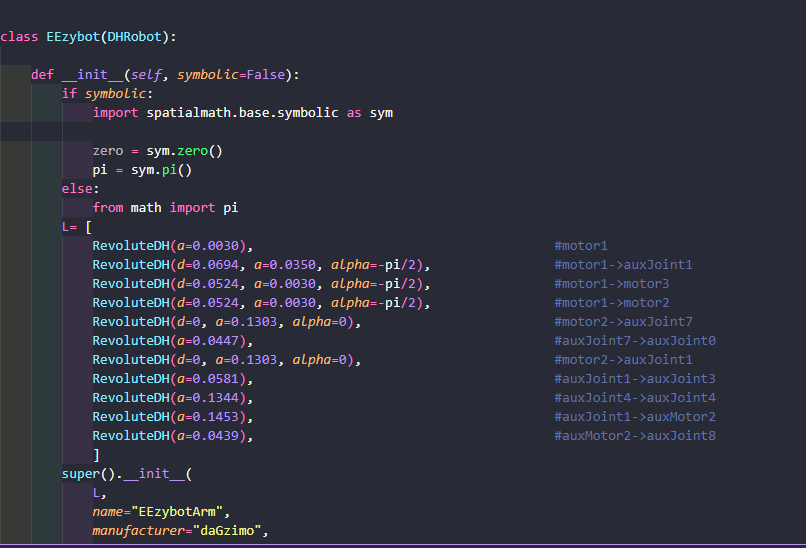
\includegraphics[scale=0.6]{img/dh.png}
		\end{center}
        \legend{\textbf{Fonte:} Autoria própria}
	\end{figure}

A descrição foi feita frame a frame, levando em conta todos os elos e juntas do robô. Por meio do método plot() é possivel visualizar um esboço dos elos e juntas do manipulador descrito (Fig. \ref{img:eezybot_dhcompleto.png}):

\imagem{0.6}{eezybot_dhcompleto.png}{EEzybotArm.plot() conforme foi descrito}{Autoria própria}

Com base no texto de \cite{Siciliano2009}, uma forma de analisar uma cadeia fechada é abrindo virtualmente a junta que une e fecha a cadeia, e analisar separadamente as duas cadeias que se formam, uma curta e outra longa.  Seguindo essa metodologia, outras formas de descrever o EEzybotArm no RTB foram pensadas e aplicadas, como visto nas figuras \ref{img:eezybot_dhshort} e \ref{img:eezybot_dhlong}. E ao descrever o manipulador essa forma, os plots dos manipuladores são gerados conforme as figuras \ref{img:eezybot_dhshort_plot} e \ref{img:eezybot_dhlong_plot}.

\begin{figure}[!htbp]
\centering
    \caption{\label{img:figura23} Parâmetros de DH do manipulador}
    \subcaptionbox{\label{img:eezybot_dhshort} DH para a cadeia curta do EEzybotArm}{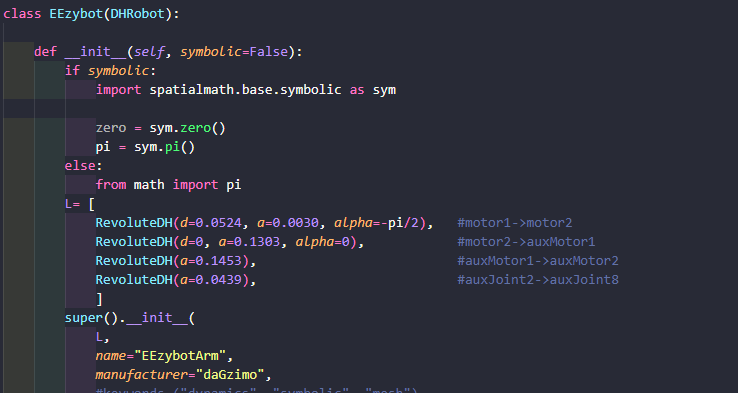
\includegraphics[scale=.5]{img/eezybot_dhshort.png}}
    \subcaptionbox{\label{img:eezybot_dhlong} DH para a cadeia longa do EEzybotArm}{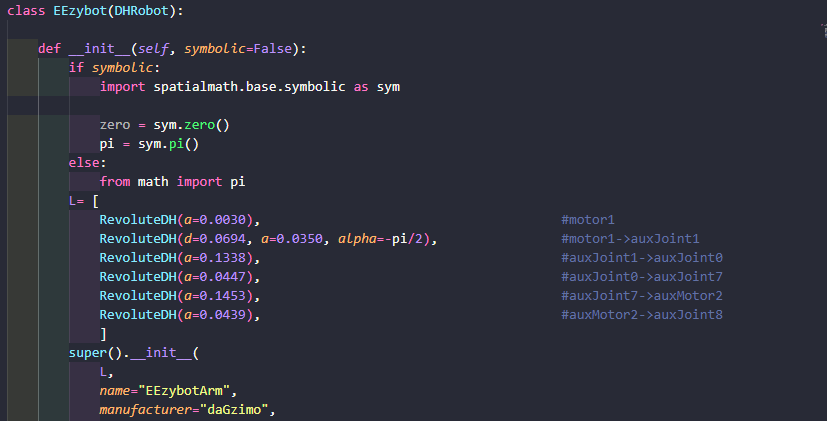
\includegraphics[scale=.5]{img/eezybot_dhlong.png}}
    \vspace{1.5em}
    \legend{\textbf{Fonte:} Autoria própria}
\label{fig:dag}
\end{figure}

\begin{figure}[!htbp]
\centering
    \caption{\label{img:figura23b} Parâmetros de DH do manipulador}
    \subcaptionbox{\label{img:eezybot_dhshort_plot} Plot para a cadeia curta do EEzybotArm}{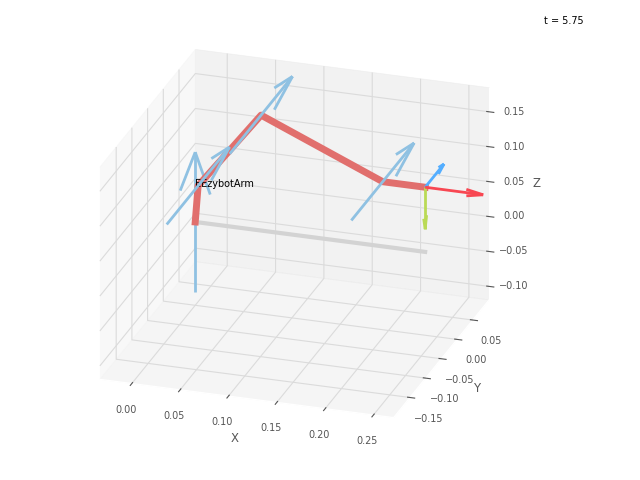
\includegraphics[scale=.55]{img/eezybot_dhshort_plot.png}}
    \subcaptionbox{\label{img:eezybot_dhlong_plot} Plot para a cadeia longa do EEzybotArm}{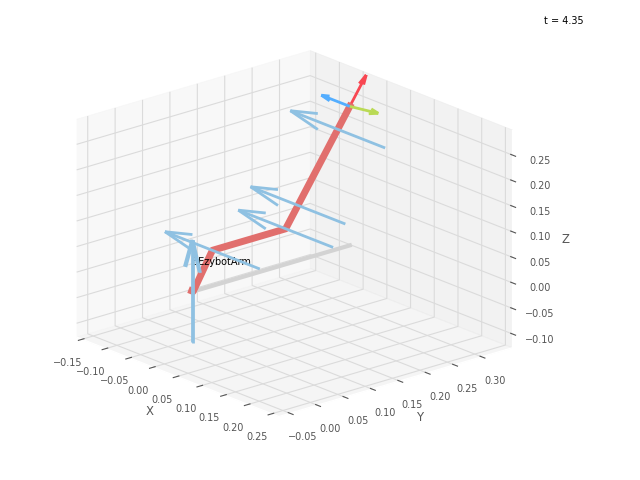
\includegraphics[scale=.55]{img/eezybot_dhlong_plot.png}}
    \vspace{1.5em}
    \legend{\textbf{Fonte:} Autoria própria}
\label{fig:dag}
\end{figure}

O repositório no Github easyEEZYbotArm do @meisben \cite{MoneyCoomes2021} disponibiliza um controlador python e arduino para o EEZYbotARM Mk1 e Mk2, incluindo cinemática nas três dimensões. Investigando os códigos, a função que implementa a cinemática inversa segue o método geométrico aplicado por \cite{costa2017}, chegando aos mesmos resultados. Então unindo o CoppeliaSim a esses scripts em python foi possível estabelecer uma comunicação satisfatória entre os dois ambientes (Fig. \ref{img:figura24.png}). Apenas as funções de cinemática inversa e plot foram utilizadas do projeto easyEEZYbotArm. 

\imagem{0.5}{figura24.png}{EEzybotArm: Plot no python e simulação no CoppeliaSim}{Autoria própria}



%--------------------------------------------------------------------------------------
% Insere a seção de cronograma
% Está comentada porque só é necessária no TCC I
%--------------------------------------------------------------------------------------
%\section{Cronograma TCC II}
%
%A continuidade desse projeto se dará da seguinte forma:
%\begin{itemize}
%	\item Com base no modelo CAD, os parâmetros de Denavit-Hartenberg serão obtidos, para
%então realizar a análise da cinemática direta e da cinemática inversa do manipulador;
%	\item As partes serão impressas, e o manipulador, montado;
%	\item O controle do manipulador será desenvolvido e implementado no arduino uno;
%	\item Testes e experimentos serão realizados a fim de comparar os resultados obtidos com
%os dados encontrados nas análises de cinemática;
%	\item Publicar os resultados em repositórios, a fim de compartilhar com a comunidade
%entusiasta do faça você mesmo dados cinemáticos e dinâmicos de um projeto tido
%como amador.
%\end{itemize}
%
%\newpage
%\section{Cronograma} \label{sec:crono}
%
%A tabela \ref{tab:cronograma} mostra o cronograma de atividades a serem executadas para o TCC II, com ênfase no calendário de 2022.1 da UNIVASF.
%
%\begin{table}[!thb]
	%\huge
	%\centering
	%\caption{\label{tab:cronograma} Cronograma das atividades previstas para o TCC II}
	%\begin{adjustbox}{max width=\textwidth}
		%\begin{tabular}{|l|l|l|l|l|l|}
			%\toprule
			%\textbf{Atividade}									& Out & Nov & Dez & Jan & Fev \\ \hline
		%	Analise Cinemática com RTB                          & x   & x   &     &     &     \\ \hline
		%	Montar manipulador impresso                         &     & x   & x   &     &     \\ \hline
	%		Modelagem do controlador e implementação no Arduino &     &     &     & x   &     \\ \hline
	%		Testes e simulações                                 &     &     &     & x   & x   \\ \hline
	%		Escrita do TCC II                                   & x   & x   & x   & x   & x   \\ \hline
	%		Defesa do TCC II                                    &     &     &     &     & x   \\ \hline
	%		\end{tabular}
%	\end{adjustbox}
%	\legend{\textbf{Fonte:} Autoria própria.}
%\end{table}

